\paragraph{Метод трассировки лучей}
Рассмотрим выпуклый многоугольник. Необходимо определить, находится ли заданная точка внутри него. Алгоритм можно описать следующим образом:
\begin{enumerate}
	\item Из тестируемой точки выпускается луч либо в заранее заданном, либо в произвольном направлении;
	\item Считается количество пересечений с многоугольником;
	\item Если количество пересечений четное, точка находимся снаружи. Если количество пересечений нечетное, точка – внутри (см. Рисунок \ref{trace_method});
\end{enumerate}
\begin{figure}[H]
	\centering
	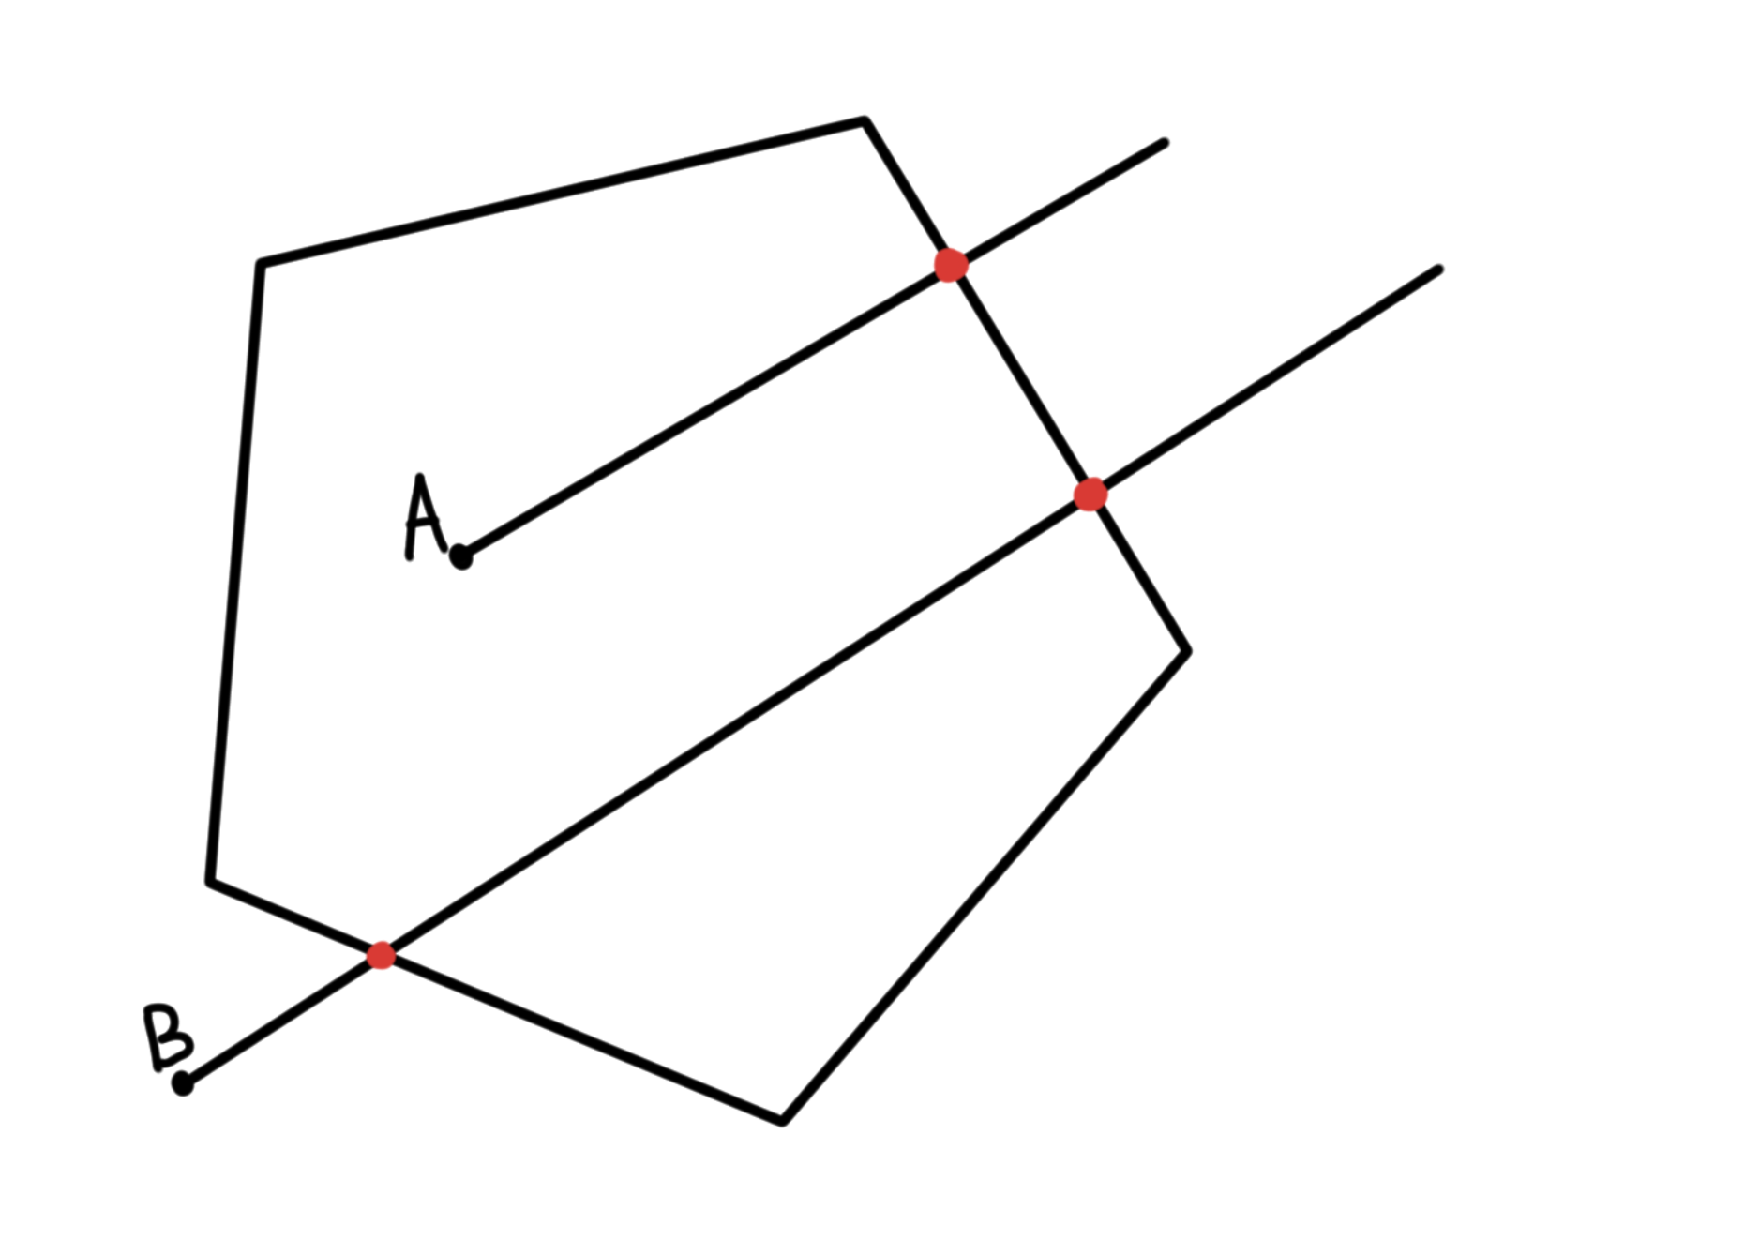
\includegraphics[width=.6\linewidth,trim={2cm 2cm 5cm 2cm}]{img/gmtrace}
	\caption{Применение трассировки для решения задачи принадлежности точки многоугольнику. Для точки $A$ найдено одно пересечение (следовательно, она внутри), для точки $B$ найдено два пересечения (следовательно, она снаружи)}
	\label{trace_method}
\end{figure}
\lstinputlisting[language=C++, firstline=159, lastline=172]{current-lines/src/Element/Element.cpp}
Полное описание метода см. \cite{pnpoly}.